\section{Reingeniería de software}

La necesidad de la reingeniería parte por un \textbf{diagnóstico}:
una aplicación que lleva años en uso,
mantenida y ampliada por diferentes equipos,
y que, por los motivos que fueran, 
deja de lado las buenas prácticas señaladas.
Esta aplicación se vuelve, en dicho contexto, \textbf{inestable},
y por lo tanto candidata a atravesar un proceso de \textbf{reingeniería}.

Frente a esta situación, Pressman señala la importancia de abordar 
el problema desde una \textbf{perspectiva pragmática},
proponiendo para ellos un modelo para el proceso de reingeniería,
que se ilustra a continuación:

\vspace{.5cm}
\begin{figure}[H]
    \centering
    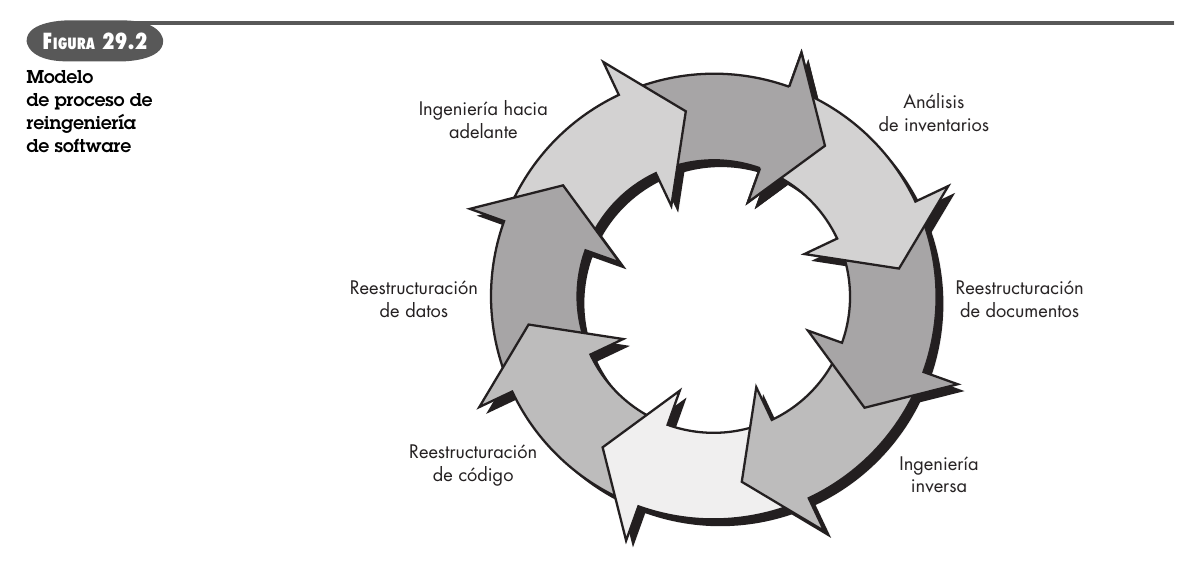
\includegraphics[width=.95\textwidth]{modelo-reingenieria.png}
    \caption{Modelo de Reingeniería de Software}
\end{figure}
\vspace{.5cm}

Se trata de un \textbf{modelo cíclico},
cuyas etapas pueden atravesarse de manera iterativa
(o saltearse por completo, como veremos, dependiendo del problema en cuestión).

Las etapas propuestas son:
\begin{enumerate}
    \item Análisis de inventarios
    \item Reestructuración de documentos
    \item Ingeniería inversa
    \item Reestructuración del código 
    \item Reestructuración de datos 
    \item Ingeniería hacia adelante
\end{enumerate}

En las secciones siguientes veremos con detenimiento cada una de estas etapas,
así como las propuestas concretas que hace el autor respecto de cada una.